\documentclass[12pt, titlepage]{article}

\usepackage{fullpage} %full page typesetting
\usepackage{setspace} %allows for non-singlespacing
\usepackage{graphicx} %graphics capabilities
\usepackage{latexsym} %extra symbols
\usepackage{rotating} %rotation for figures
\usepackage{longtable} %tables that fill more than a single page
%\usepackage{hyperref} %hypertext links in the document
\usepackage{natbib} %better bibliographies
\usepackage{authblk} %author and affiliation in opening
\usepackage{mathpazo} %use palatino font, rather than times
\usepackage{appendix}
\usepackage{lscape}
\usepackage{tabulary}
\usepackage[nottoc]{tocbibind}
\usepackage[colorlinks=true,linkcolor=blue,citecolor=cyan]{hyperref}
\usepackage{ifthen}

\title{\tb{Place of Residence and Political Attitudes in Democracies Worldwide }}

\author{Jennifer Lin}
\affil{New College of Florida}

\newcommand\e{\emph}
\newcommand\tb{\textbf}
\newcommand\un{\underline}
\newcommand\txt{\texttt}

\doublespacing 

\begin{document}

\begin{singlespace}
\maketitle
\end{singlespace}

\begin{center} %center text
\section*{Abstract} %the star stops this section from appearing in the ToC
	
\begin{quote}
After the 2016 election, many major new pundits pointed at Rural America as the major source of Donald Trump’s victory for the presidency. This is because, as prior research by \cite{walsh_putting_2012} for the United States and \cite{walks_city-suburban_2005} for Canada suggests, residents in rural parts of democratic countries tend to be more religious and less exposed to diversity as their urban counterparts. As a result, they are more conservative in their social views even if they may be more liberal on their fiscal ones. President Trump took advantage of this and won the hearts and minds of many voters in the Midwest and Rural South, which allowed him to secure an electoral college victory despite falling short on the popular vote. For this research project, I was interested to see if this trend extends to other developing and consolidated democracies in the world. Using the CSES Module IV data (2011-2016), I conducted regressions to test place of residence on a self-defined ideological scale and an objective ideology scale constructed using respondent opinions on various issues. By controlling for regime factors such as age and level of democracy, I find statistical significance to suggest that place matters. The data provides sufficient evidence to suggest that if one lives in an urban place compared to a rural one, they are more likely to self-identify as more liberal and hold those values when voicing their opinions on social issues.

\end{quote}
\end{center}

\clearpage

\tableofcontents
%\addcontentsline{toc}{section}{\listfigurename}
%\addcontentsline{toc}{section}{\listtablename}
\clearpage

\listoftables
\clearpage

\listoffigures
\clearpage

\section{Introduction}

After the election of Donald Trump as the 45th President of the United States, news pundits speculate that the reason for his election was through the support that he won from rural voters in the South and Midwest. These Republican strongholds located in the rural and suburban parts of the country have been researched by political scientists \citep{walsh_putting_2012} and the results suggest that there is an urban-rural divide that is growing in the United States. Additionally, it is noticeable that the mindset of individuals who live in different parts of the country do not conceptualize politics in a similar fashion \citep{holloway_burning_2007}. These differences in interests leads to differences in ideologies and attitudes, as seen in the United States back in 2016.

However, the United States does not operate in isolation and the people are not necessarily idiosyncratic compared to others around the world. Therefore, in this paper, I am interested in understanding if the urban-rural divide that is present in the US is also present and noticeable in other places around the globe. Additionally, I  will discuss how living in a different environment leads people to favor different interests and hold distinct political beliefs in the context of key regime factors such as the level of democracy, age of regime and the type of electoral formula that a regime employs in their system of government.
 
Through the analysis of the Comparative Study of Electoral Systems (CSES), I find that place of residence does matter in influencing one's political beliefs and ideologies. More specifically, the results will allow us to draw two conclusions. First, the place of residence matters in influencing political attitudes, but this is heavily influenced on the regime's electoral formula such that if a respondent lives in a first past the post system, there is a greater pronounced difference between place of residence and ideology, but this effect is not significant in proportional representation systems. Second, the influence of place of residence on political ideology is more pronounced in more established and longstanding democracies than developing ones such that the divide between urban, suburban, small town, and rural residents are more pronounced when the regime has a system of democracy that has been instituted for a longer period of time.
 
\section{Theoretical Review of Literature}

\subsection{Trends of Urban-Rural Divide in Seen in Previous Case Studies}



\subsection{Connections between Place and Political Ideology}



\subsection{Polities in this Study}

% Table for D1015 - election type
\begin{table}
	\centering
	%\resizebox{\columnwidth}{!}
	%\def\arraystretch{1.5}
	\caption{\tb{Types of Election by Polity}}
	\begin{tabulary}{\textwidth}{l c c c c} 
		\hline
		\tb{Country}&\tb{Year}&\tb{Legislative}&\tb{Both}&\tb{Presidential}\\
		\hline
		Argentina&2015&-&X&-\\
		Australia&2013&X&-&-\\
		Austria&2013&X&-&-\\
		Bulgaria&2014&X&-&-\\
		Czech Republic&2013&X&-&-\\
		Finland&2015&X&-&-\\
		France&2012&-&-&X\\
		Germany&2013&X&-&-\\ 
		Great Britain&2015&X&-&-\\
		Greece&2012/2015&X&-&-\\
		Iceland&2013&X&-&-\\
		Ireland&2011&X&-&-\\
		Israel&2013&X&-&-\\
		Japan&2013&X&-&-\\
		Kenya&2013&-&X&-\\
		Latvia&2011/2014&X&-&-\\
		Mexico&2012&-&X&-\\
		Mexico&2015&X&-&-\\
		Montenegro&2012&X&-&-\\
		Norway&2013&X&-&-\\
		New Zealand&2011/2014&X&-&-\\
		Peru&2016&-&X&-\\
		Philippines&2016&-&X&-\\
		Poland&2011&X&-&-\\
		Portugal&2015&X&-&-\\	
		Romania&2012&X&-&-\\
		Romania&2014&-&-&X\\
		Serbia&2012&-&X&-\\
		Slovakia&2016&X&-&-\\
		Slovenia&2011&X&-&-\\
		South Africa&2014&X&-&-\\ 
		South Korea&2012&X&-&-\\
		Sweden&2014&X&-&-\\
		Switzerland&2011&X&-&-\\
		Turkey&2015&X&-&-\\
		\hline
	\end{tabulary} \\
	\e{Source:} Comparative Study of Electoral Systems Module IV 
	\label{table1}
\end{table}

%Brazil&2014&-&X&-\\
%Canada&2011&X&-&-\\
%Canada&2015&X&-&-\\
%Hong Kong&2012&X&-&-\\
%United States&2012&-&X&-\\
%Taiwan&2012&-&X&-\\
%Thailand&2011&X&-&-\\

Table \ref{table1} shows the types of elections that are held within each of the polities that are represented in the Comparative Study of Electoral Systems Module IV data. From this table, we see that many of the countries are holding legislative, or parliamentary elections to some extent during the period between 2011 and 2016

%Table for D2031 by polity

Table \ref{table2} shows the percentage of people in each polity that lives in each of the four different places of residence. 

\begin{table}[h!]
	\centering
	\caption{\tb{Percentage of People in Each Place of Residence by Polity}}
	\begin{tabulary}{\linewidth}{l c c c c}
		\hline
		\tb{Country}&\tb{Rural}&\tb{Small Town}&\tb{Suburban}&\tb{Urban}\\
		\hline
		Worldwide&26.98&22.95&13.37&36.70 \\
		Argentina&-&13.30&-&86.70 \\
		Australia&10.92&18.73&16.98&53.37 \\
		Austria&41.67&27.54&18.19&12.60 \\
		Bulgaria&26.33&20.82&36.14&16.72 \\
		Czech Republic&26.68&39.87&5.01&29.24 \\
		Germany&28.80&42.56&9.53&19.11 \\
		Finland&25.16&23.39&42.50&8.95 \\
		France&35.10&37.34&11.72&15.84 \\
		Great Britain&17.68&52.84&-&29.48 \\
		Greece (2012)&40.77&10.62&11.51&31.10 \\
		Greece (2015)&5.86&21.48&13.99&58.68 \\
		Iceland&9.06&28.87&26.17&35.90 \\
		Ireland&-&40.91&-&59.09 \\
		Israel&20.50&54.40&25.10&- \\
		Japan&12.80&25.86&17.86&43.47 \\
		Kenya&66.67&-&-&33.33 \\
		Latvia (2011)&36.75&18.13&-&45.12 \\
		Latvia (2014)&34.46&25.29&10.42&29.83 \\
		Mexico (2012)&18.33&11.67&-&70.00 \\
		Mexico (2015)&18.38&11.28&-&70.34 \\
		Montenegro&37.47&36.72&12.85&12.96 \\
		Norway&26.43&25.54&13.69&34.35 \\
		New Zealand (2011)&16.32&38.12&-&45.56 \\
		New Zealand (2014)&13.36&21.04&-&65.61 \\
		Peru&20.99&-&-&79.01 \\
		Philippines&45.00&14.58&3.33&37.88 \\
		Poland&35.85&42.57&9.64&11.93 \\
		Portugal&28.75&25.48&16.81&28.95 \\
		Romania (2012)&44.63&22.83&2.37&30.97 \\
		Romania (2015)&41.82&29.95&11.78&16.46 \\
		Serbia&49.62&24.04&9.44&16.90 \\
		Slovakia&42.38&39.16&1.48&16.97 \\
		Slovenia&22.88&12.65&49.66&14.61 \\
		South Africa&30.77&-&-&69.23 \\
		South Korea&17.00&28.40&6.00&48.60 \\
		Sweden&17.55&22.12&21.15&39.18 \\
		Switzerland&26.67&0.66&47.30&25.37 \\
		Turkey&19.06&21.64&17.96&41.34 \\
		\hline
	\end{tabulary} \\
\e{Source:} Comparative Study of Electoral Systems Module IV 
\label{table2}
\end{table}

%Thailand&76.24&3.61&4.08&16.07 \\

\begin{figure}[ht!]    \centering
	{	 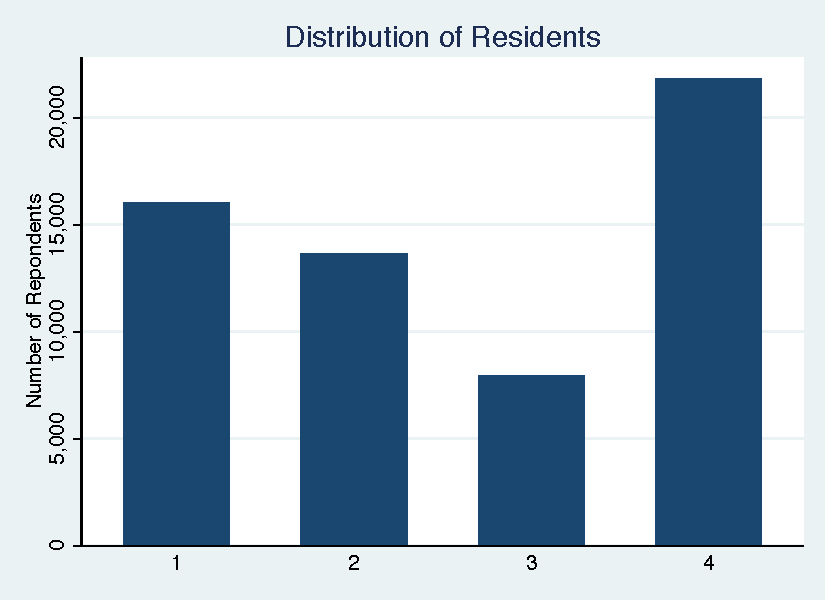
\includegraphics[width=\textwidth]{Residents}}
	\caption{\tb{Distribution of Responses By Place of Residence}}\label{figure1}
\end{figure}


\begin{figure}[ht!]    \centering
	{	 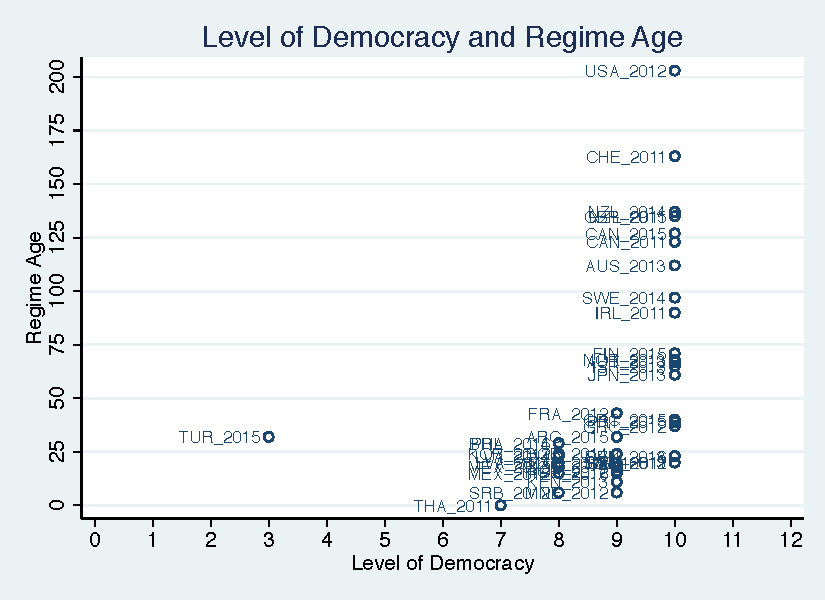
\includegraphics[width=\textwidth]{DemAge}}
	\caption{\tb{Level of Democracy and Regime Age}}\label{figure2}
\end{figure}

\subsection{Proceeding with Caution}



\section{Hypotheses}

From the review of literature, we see that there seems to be an ideological divide between people living in rural and urban areas of their respective countries. From case studies, most notably in the United States and Canada, there is a pattern such that the individuals living in rural areas tend to err towards conservatism and residents of urban centers tend to veer towards liberalism. However, given that these are relatively established democracies, I wonder how differences in levels of democratic development, regime age and other ideosyncratic factors that shape a regime influence the divide of political ideologies between urban and rural residents. Therefore, the present research will test three hypotheses relating to the relationship between the place of residence of an individual and their political ideology.

\begin{quote}
	\e {Hypothesis 1 -- Place Matters:} An individual's place of residence influences their political ideology such that the more distant the characteristics of one's vicinity gets from an urban city, the more conservative one will become.
\end{quote}

The \e{Place Matters} hypothesis suggests that there is a direct relationship between place of residence and political ideology no matter where an individual lives in this world. Therefore, this hypothesis assumes that, broadly speaking, individuals who live in a rural area will be more conservative than those who live in a small town or urban center. In this case, political ideology, as we will also see later, is operationalized by the respondent's self-placement on the ideology spectrum. Therefore, this is based on their own views on how liberal or conservative they are. While this is helpful to understand how place of residence influences political ideology, it would be even more helpful to introduce a second hypothesis that looks at objective support for policies which can show where a person lies on the political spectrum.

\begin{quote}
	\e{Hypothesis 2 -- Issue Stances:} An individual's place of residence influences the way they conceptualize pressing issures and their stances towards these issues.
\end{quote}

In the \e{Issue Stances} hypothesis, I predict that people will understand the meaning of issues differently based on where they live and hold different opinions about them as a result of their place of residence. In other words, if the \e{place Matters} hypothesis holds true, people who live in rural areas will see issues differently than those who live in urban areas and apply their political ideologies when deciding on the issues. 

Both the \e{Place Matters} and \e{Issue Stances} hypotheses assumes that countries are the same across the board and that one's conceptualization of place of residence is uniform. Therefore, in the last hypothesis, I will integrate some polity defining factors into the model to understand how certain aspects of each regime such as their level of democracy, regime age and electoral formula influence the relationships that are observed in the preceding hypotheses. 

\begin{quote}
	\e{Hypothesis 3A -- Level of Democracy:} A regime's level of democracy will influence the political ideologies of citizens based on their place of residence such that the influence of place on political ideology will increase as a regime becomes more democratic. 
	
	\e{Hypothesis 3B -- Regime Age:} A regime's age will influence the political ideologies of citizens based on their place of residence such that the relationship between place of residence and political ideology will be more pronounced when the regime is older
	
	\e{Hypothesis 3C -- Electoral Formula:} A regime's method of elections will influence the political ideologies of citizens based on their place of residence such that pluralistic, first past the post systems will increase the influence of place of residence on political ideologies.
	
	\e{Hypothesis 3D -- Polity Differences} The regime's level of democracy, age and electoral formula will cooperate to determine the extent to which place of residence can influence political ideology in a given polity.
\end{quote}

Each of the components embedded in Hypothesis 3 analyzes key differences in how each polity functions and the stability of democracy such that a more stable democracy can mean more room for an individual to consider their true self-interests rather than being forced to believe something as a means of survival. In each of the sections of Hypothesis 3, we analyze how the successful consolidation of democracy, or lack thereof, influences how other social factors, such as place of residence, can influence a person's political views. I include the age of the regime to identify if a longer lasting polity can solidify the patterns of influence that place of residence has on an individual's political outlook and stance on issues. Finally, I include the electoral formula as a means of understanding how the system of representation influences the relationship between the core variables used in this paper. For the \e{Electoral Formula} hypothesis, I hypothesize that if individuals had to fight for representation in a winner take all system, personal factors such as place of residence will be more salient than if all interests were more fairly represented in a proportional system. Each of these components are then tied together to understand how idiosyncrasies of a polity lead to the difference between place of residence and political ideology as explored in the \e{Place Matters} and the \e{Issue Stances} hypotheses.

Through the research, we will be able to see whether there is a relationship across the globe surrounding place of residence and political ideology. In the following sections, I explain the models that will be used to understand the relationships between the variables. We will revisit the hypotheses in the discussion to see if the data supports them along with possible limitations that may be present.

\section{Research Design}

\subsection{Data}

To understand the divide between rural and urban residents in different countries of the world, I will consider cases analyzed in the Comparative Study of Electoral Systems (CSES) Module IV dataset for the analysis of these trends. In this specific module, the CSES considers elections that occurred between 2011 and 2016 in various democracies around the world. In the following sections, I will describe the variables used in this project in more detail. Each of the variable names and descriptions are also located in Appendix \ref{AppendixA}, which contains the variable code referenced in the CSES dataset.

\subsection{Key Independent Variables}

In this data analysis, the key independent variables that are considered include the respondent's country and place of residence. For this analysis, place of residence is considered to be based on the categories that are established by the survey such that individuals either live in a rural village, small town, suburbs of a large city or within the large city itself. In the regression model, this variable is characterized as a category even though there are places that may be in between two of the categories that characterize place of residence. 

Each individual's country of residence is also classified based on the year of the election, level of democracy during the election year,  age of the current governing regime in the country at the time of the election, and the type of electoral formula employed by the governing body to determine winners of seats in government. The level of democracy is characterized by how free the polity is at the time of the election. This measure was gathered from the generators of the Polity IV project and reflects freedom from a -10 to 10 scale with -10 being the most autocratic and 10 being the most democratic. The age of the current governing regime suggests how long the current system has been in power. The larger value suggests that the current system in government has been established for a longer period of time and is therefore more stable. Finally, the type of electoral formula describes how government official win office based on their total vote share. Contestants may win via majoritarian, proportional or mixed system. 

\subsection{Key Dependent Variables and Measures}

To understand where individuals see their own political values, the dependent variable reflects their self-identified ideology, a variable coded by the CSES that ranges from 0 to 10 with 0 being the most left leaning and 10 as the most right leaning ideological stance.. Since this can be rather subjective, i also created a liberalism scale that reflects individual values on government spending with a more liberal vision being those who value spending for social benefits and a more conservative view for those who do not with for such spending or for those who wish to spend more to boost defence as a means to secure their country's identity and values. (See Appendix \ref{AppendixB} for a more detailed description of this scale creation) This 9-point scale was generated from questions relating to public expenditure used in the survey. Topics for these questions include health, education, unemployment benefits, defense, old age pensions, business and industry investments, police and law enforcement and welfare benefits. Additionally, I add a value of economic equality to the measure as a means of understanding how each person values equality as part of their ideological outlook. This scale ranges from 0 to 9, with 0 being the most conservative and 9 being the most liberal. In the broadest context, respondents who score at the extreme ends of the scale are seen to be most conservative or liberal in terms of their outlook on spending, which can speak to their views on social values given their willingness to allocate government money to these groups.

\subsection{Models for Analysis}

In this study, I will utilize five different regression analyses for each of the two dependent measures to uncover patterns in the data and help answer the guiding questions posed in the introduction. I will utilize the variables discussed in the previous sections to find connections between place of residence and political ideologies.

The first regression will consider the core of the \e{Place Matters} hypothesis. I will regress the place of residence variable on the respondent's self-placement on the political ideology scale. The second, third and fourth regressions will factor in the effects of a country's level of democracy, regime age, and electoral formula at the time of the election into the picture to observe their influences on the relationship in the \e{Place Matters} hypothesis. A fifth regression will be employed to understand how the inclusion of all the variables influences the first hypothesis. These subsequent hypotheses are aimed at testing the components of Hypothesis 3.

Hypothesis 2, or the \e{Issue Stances} hypothesis, is constructed as an objective measure and check to the subjective ratings. The Liberalism scale will be a dependent measure on another series of regressions that mirror the first set. The major difference with this set of regressions from the preceding set is the differences in dependent measure such that the former is based on how individuals think they are placed on the political ideology spectrum based on self-judgment, the latter is the measure of ideology based on the individual's actual policy stances.

In the following section, I discuss the results for the regressions and comment on the observations that these regressions can suggest for the relationship between place of residence and political ideology across a sample of countries across the world.

% Cross tabulate liberalism and self ideology to see how the two line up
\section{Results}



\subsection{Self-Placement Ideology as a Dependent Measure}

\begin{table}
	\centering
	\def\arraystretch{1.5}
	\caption{\tb{Self-Placement Ideology - Worldwide}}
	\begin{tabulary}{\linewidth}{l c}
		\\
		\hline
		\tb{Place of Residence}&\tb{Worldwide} \\
		\hline
		Small Town&-.1338***  \\    
		  & (.0336)   \\
		Suburban & -.2591***\\ 
		 & (.0358) \\
		Urban   & -.0482   \\
		  & (.0300)    \\
		Constant   & 5.597***  \\
		&(.0234) \\
		N  & 47,821  \\
		$R^2$	& 0.0011 \\
		\hline                                       
    \end{tabulary}
\\
\e{Notes:} *p$<$.1, **p$<$.05. ***p$<$.01 \\
\e{Reference:} A rural place of residence serves as the baseline for comparison
\label{table3}
\end{table}

\begin{table}
\centering
\def\arraystretch{1.5}
\caption{\tb{Self-Placement Ideology - Central/Latin America}}
	\begin{tabulary}{\linewidth}{l c c c c}
	\\
	\hline
	\tb{Place of Residence}&\tb{Argentina}&\tb{Mexico (2012)}&\tb{Mexico (2015)} &\tb{Peru}\\
	\hline
	Small Town  & -    & .6408***   &-.4734    & -   \\      
	  & -  & (.2394) & (.3113)    & -    \\
	Suburban    & -    & -   & -   & -    \\ 
	& -     & -    & -   & -    \\
	Urban   & -.9521*** & -.1417   & -.4084*   & .0883  \\
	   & (.2150)   &(.1678)   & (.2210)  & (.1743)      \\
	Constant   & 6.495*** & 6.6516*** & 6.1690*** & 6.646***   \\
	&(.2046)&(.1493)&(.1998)&(.1564) \\
	N  & 1,241 &1,812   & 910 & 1,438   \\
	$R^2$ & 0.0156   &0.0082   &0.0041 &0.0002     \\
	\hline                                       
	\end{tabulary} 
\\
\e{Notes:} *p$<$.1, **p$<$.05. ***p$<$.01 \\
\e{Reference:} A rural place of residence serves as the baseline for comparison
\label{table4}
\end{table}

\begin{landscape}
\begin{table}
	\centering
	\def\arraystretch{1.5}
	\caption{\tb{Self-Placement Ideology - Western Europe}}
	\begin{tabulary}{\linewidth}{l c c c c c c}
		\\
		\hline
		\tb{Place of Residence}&\tb{Switzerland}&\tb{Germany}&\tb{France} &\tb{Great Britain}&\tb{Ireland}&\tb{Portugal}\\
		\hline
		Small Town   & - .4973  & -.3295*** &-.1148 &  -.3773***  & -   &-.3717* \\      
		& (.4333)  & (.1087)  & (.1321)    & (.1392)  &- & (.2157) \\
		Suburban  & -.2663***   & .0912 & -.0246  & -      &-    & -1.1139*** \\ 
	    & (.0852)  & (.1693)  & (.1886)   & -      & - & (.2421)  \\
		Urban  & -.8650***  & -.6361*** & -..7254***  & -.8310***      &-.2494**& -.8348***   \\
	    & (.0976)  &(.1311)  & (.1706)    & (.1538)   & (.0986)  & (.2121)  \\
		Constant & 5.462***  & 4.630***  & 4.8086***  & 5.3992***  & 6.1491***  &5.4661***   \\
		&(.0681)&(0.0845)&(.0943)&(.1197)&(.0772)&(.1483) \\
		N  & 4,728    &1,697  & 1,916  & 1,386     &  1,594  &1,224  \\
		$R^2$  & 0.0191    &0.0176 &0.0102    &0.0217  &  0.0040 &0.0218  \\
		\hline                                       
	\end{tabulary} 
	\\
	\e{Notes:} *p$<$.1, **p$<$.05. ***p$<$.01 \\
	\e{Reference:} A rural place of residence serves as the baseline for comparison
	\label{table5}
\end{table}
\end{landscape}

\begin{table}
	\centering
	\def\arraystretch{1.5}
	\caption{\tb{Self-Placement Ideology - Scandinavia}}
	\begin{tabulary}{\linewidth}{l c c c c}
		\\
		\hline
		\tb{Place of Residence}&\tb{Finland}&\tb{Iceland}&\tb{Norway}&\tb{Sweden} \\
		\hline
		Small Town&.1418&.5194**&.0568&-.1030 \\
		&(.1646)&(.2279)&(.1534)&(.2644) \\
		Suburban&-.0612&.7355***&-.0277&.0794 \\
		&(.1452)&(.2290)&(.1847)&(.2690) \\
		Urban&-.7128***&.3840*& .0888&-.1723\\
		&(.2202)&(.2220)&(.1429)&(.2368) \\
		Constant&5.6503***&4.990***&5.5985***&5.2230*** \\
		&(.1169)&(.2006)&(.1080)&(.1973) \\
		N&1,387&1,266&1,618&792\\
		$R^2$&0.0111&0.0096&0.0004&0.0018 \\
		\hline
	\end{tabulary}
\\
\e{Notes:} *p$<$.1, **p$<$.05. ***p$<$.01 \\
\e{Reference:} A rural place of residence serves as the baseline for comparison
\label{table6}
\end{table}

\begin{table}
	\centering
	\def\arraystretch{1.5}
	\caption{\tb{Self-Placement Ideology - Central Europe}}
	\begin{tabulary}{\linewidth}{l c c c c c}
		\\
		\hline
		\tb{Place of Residence} &\tb{Austria}&\tb{Czech Republic}& \tb{Poland} &\tb{Slovakia}&\tb{Slovenia} \\
		\hline
		Small Town&-.2108& -.0223 & .0829 & .4318*** & .0229 \\
		&(.1540) & (.1687) & (.1421) & (.2000) & (.3262)\\
		Suburban&-.1433& -.6091*& -.1414 & 1.059& .1549** \\
		&(.1570)&(.3281) & (.2210) & (.6711) & (.2491)\\
		Urban&-.3005**&.2860 & -.2002 & .8061*** & -1.3416***\\
		&(.1335) &(.1773) & (.2042) & (.2437) & (.3169)\\
		Constant& 5.3726***& 4.9135***& 6.015*** & 4.7527***  & 4.6780 ***\\
		&(.1219) & (.1300) & (.1050) & (.1370) & (.2060)\\
		N&3,363& 1,412& 1,634 & 879& 666 \\
		$R^2$&0.0018&0.0065 & 0.0016 & 0.0148 & 0.0629\\
		\hline
		\end{tabulary}
	\\
	\e{Notes:} *p$<$.1, **p$<$.05. ***p$<$.01 \\
	\e{Reference:} A rural place of residence serves as the baseline for comparison
	\label{table7}
	\end{table}

\begin{landscape}
\begin{table}
	\centering
	\def\arraystretch{1.5}
	\caption{\tb{Self-Placement Ideology - Southwestern Europe}}
	\begin{tabulary}{\linewidth}{l c}
		\\
		\hline
		\tb{Place of Residence}& \tb{Bulgaria} \\
		\hline
		Small Town&.5324 \\
		&(.3313) \\
		Suburban& .7821*** \\
		& (.2914) \\
		Urban& .8838** \\
		& (.3590) \\
		Constant& 4.739 *** \\
		& (.2267) \\
		N& 750 \\
		$R^2$&0.0118 \\
		\hline
	\end{tabulary}
\\
\e{Notes:} *p$<$.1, **p$<$.05. ***p$<$.01 \\
\e{Reference:} A rural place of residence serves as the baseline for comparison
\label{table8}
\end{table}
\end{landscape}

\begin{landscape}
\begin{table}
	\centering
	\def\arraystretch{1.5}
	\caption{\tb{Self-Placement Ideology - Pacific Islands}}
	\begin{tabulary}{\linewidth}{l c c c c}
		\\
		\hline
		\tb{Place of Residence}&\tb{Australia}&\tb{New Zealand (2011)}&\tb{New Zealand (2014)} &\tb{Philippines}\\
		\hline
		Small Town  & - .2108  & -.2283  &-.1436 &  .6419***  \\      
		& (.1540)   & (.2213) & (.2864)  & (.2060)    \\
		Suburban  & -.1433   & -   & -    & - .1095   \\ 
		& (.1570)   & -  & -    & (.3871)       \\
		Urban  & -.3005** & -.2653  & -.2151 & .3048** \\
		& (.1335) &(.2114)   & (.2406) & (.1526)      \\
		Constant   & 5.372***   & 5.754*** & 5.9674***  & 7.009***   \\
		&(.1219)&(.1826)&(.2207)&(.1030) \\
		N 	 & 3,363   &1,039    & 957   & 1,179  \\
		$R^2$  & 0.0018   &0.0016  &0.0035  &0.0097     \\
		\hline                                       
	\end{tabulary} 
	\\
	\e{Notes:} *p$<$.1, **p$<$.05. ***p$<$.01 \\
	\e{Reference:} A rural place of residence serves as the baseline for comparison
	\label{table10}
\end{table}
\end{landscape}

\subsection{Objective Issue Stances as a Dependent Measure}



\section{General Discussion and Conclusion}

From the results of the data analyses, we can see that...

\subsection{Summary of Findings}


\subsection{Limitations and Future Directions}

\clearpage


\let\svaddcontentsline\addcontentsline
\renewcommand\addcontentsline[3]{%
	\ifthenelse{\equal{#1}{lof}}{}%
	{\ifthenelse{\equal{#1}{lot}}{}{\svaddcontentsline{#1}{#2}{#3}}}}


\appendixtitleon
\appendixtitletocon

\begin{appendices}

\begin{landscape}
\section{Descriptions of Variables }
\label{AppendixA}

~~~\\\\

\begin{table}[h!]
	\centering
	\def\arraystretch{1.5}
	\caption{\tb{Variables Used in Analyses}}
	\begin{tabulary}{\linewidth}{l c c c}
		\\
		\hline
		\tb{Variable Name}& \tb{Variable Number} & \tb{Description}&\tb{Outside Source} \\
		\hline
		Election ID Variable &D1004&Polity and Election Year&-\\
		Place of Residence&D2031&Rural or Urban Residence&-\\
		Left-Right Self&D3014&Self-rate ideology &-\\
		Level of Democracy&D5051\_1&Democracy-Autocracy at Election&Polity IV Project\\
		Age of Current Regime&D5052&Age of Regime in Years& Polity IV Project\\
		Electoral Formula&D5058&Method of Election&CSES Macro Report\\
		\hline
	\end{tabulary}\\
	\e{Source:} Comparative Study of Electoral Systems Module IV Codebook available at \url{http://www.cses.org/datacenter/module4/data/cses4_codebook_part2_variables.txt}
	\label{table99}
\end{table}

\begin{table}[h!]
	\centering
	\def\arraystretch{1.5}
	\caption{\tb{Issue Stances/Liberalism Scale Variables}}
	\begin{tabulary}{\linewidth}{l c c c}
		\\
		\hline
		\tb{Variable Name}& \tb{Variable Number} & \tb{Description}\\
		\hline
		Health&D3001\_1&More or Less Public Expenditure on Health\\
		Education&D3001\_2&More or Less Public Expenditure on Education\\
		Unemployment Benefits&D3001\_3&More or Less Public Expenditure on Unemployment\\
		Defense&D3001\_4&More or Less Public Expenditure on Defense\\
		Old-Age Pensions&D3001\_5&More or Less Public Expenditure on Pensions\\
		Business and Industry&D3001\_6&More or Less Public Expenditure on Businesses\\
		Police&D3001\_7&More or Less Public Expenditure on Law-Enforcement\\
		Welfare Benefits&D3001\_8&More or Less Public Expenditure on Welfare\\
		Income Inequality&D3004&Should Government do more for Income Inequality?\\
		\hline
	\end{tabulary}\\
	\e{Source:} Comparative Study of Electoral Systems Module IV Codebook available at \url{http://www.cses.org/datacenter/module4/data/cses4_codebook_part2_variables.txt}
	\label{table100}
\end{table}

\end{landscape}
\clearpage

\section{Creation of the Issue Stances/Liberalism Scale}
\label{AppendixB}

\end{appendices}


\clearpage
\bibliography{RuralPolitics}
\bibliographystyle{chicago}


\end{document}
